\begin{document}
\maketitle

\begin{abstract}
Automatic recognition of circuit schematic diagrams is a core challenge in Electronic Design Automation (EDA), involving two heterogeneous tasks: visual text extraction and topological graph tracing. This paper presents CircuitOCR, a circuit schematic OCR and netlist extraction system based on PaddleOCR-VL-0.9B. We construct the V5 Golden purified dataset, comprising 1,857 programmatically generated and real-world open-source schematics (500 synthetic renderings + 1,357 KiCad diagrams) with 100\% visual-literal alignment, split 90/10 into training (1,554) and validation (171) sets. Through systematic LoRA ablation experiments, we identify the \textbf{root cause of modality collapse}---fine-tuning the vision-language projector (\texttt{mlp\_AR}) with LoRA destroys pre-trained alignment weights---and propose the LLM-Only LoRA architecture that completely resolves this issue. The final V9-Pure model adopts a wide LoRA configuration ($r=16$, $\alpha=32$, 5.7M trainable parameters). By fixing two critical issues---causal token shift and BPE boundary merging---and training for 3 epochs (1,165 steps) on the V5 Golden purified dataset, it achieves Avg.\ NED = 0.7797 on the easy100 pure test set (baseline 0.9390, 17.0\% relative error reduction) and 0.7869 on easy50 (baseline 0.9424, 16.5\% relative error reduction). Training completes in approximately 34 minutes on a single NVIDIA RTX 4060 laptop GPU (8\,GB VRAM). Model weights, datasets, and an online demo are fully open-sourced.
\end{abstract}

\keywords{Circuit Schematic \and OCR \and PaddleOCR-VL \and LoRA Fine-tuning \and Netlist Extraction \and Modality Collapse \and Low-VRAM Training}


\section{Introduction}

\subsection{Research Background and Scarcity}

Vision-Language Models (VLMs) have substantially expanded the application boundaries of traditional large language models, demonstrating significant advantages in scenarios requiring visual understanding, such as robotic navigation and document parsing. Compared to traditional OCR pipelines that rely on multi-stage processing and substantial memory overhead, VLMs can directly output structured text from images in an end-to-end manner.

In the Electronic Design Automation (EDA) domain, automatic recognition and parsing of circuit schematic diagrams remains a research-scarce direction. Numerous general-purpose OCR benchmark datasets exist (e.g., ICDAR series, SROIE, FUNSD), covering natural scene text, documents, receipts, and forms, yet no dedicated public benchmark exists for circuit schematic OCR. Existing circuit-related datasets such as Open Schematics~\citep{openschematics2025} provide circuit diagrams and netlists but lack standardized evaluation protocols, and their original annotations suffer from format mismatch and noise. Textbook datasets, on the other hand, suffer from systematic visual-to-logic annotation discrepancies due to SPICE implicit nodes. CircuitOCR fills this gap by constructing the first format-aligned, zero-AI-label, purified circuit schematic OCR benchmark (V5 Golden Purified), comprising 1,857 high-quality samples split 90/10 for training/validation (1,554/171), with a 3-tier difficulty evaluation system.

\subsection{Industry Demand Value}

Automatic circuit schematic recognition is a core requirement in the EDA industry. According to SEMI and WSTS statistics, the global semiconductor market exceeded \$600 billion in 2025, while the PCB design tools market (Cadence, Altium, KiCad, etc.) is approximately \$4 billion. In actual engineering workflows, substantial demand exists for converting schematic diagrams from paper or image format into digital netlists:

\begin{enumerate}[nosep]
    \item \textbf{Reverse Engineering}: Hardware security audits and compatibility design require recovering original netlists from physical PCBs or images;
    \item \textbf{Legacy Document Digitization}: Large volumes of paper schematics from the 1980s--2000s require digital archiving;
    \item \textbf{Cross-Tool Migration}: Schematic formats across different EDA tools are mutually incompatible; image-level OCR can serve as a universal migration bridge;
    \item \textbf{Open-Source Hardware Community}: Over 500,000 KiCad/EAGLE projects exist on GitHub, many lacking structured netlist exports.
\end{enumerate}

Currently, these tasks primarily rely on manual image-by-image reading and entry, which is extremely inefficient and error-prone. Industry estimates suggest the PCB reverse engineering outsourcing market alone exceeds \$500 million annually, with approximately 30\% of time spent on schematic reconstruction.


\section{Background and System Setup}
\label{sec:headings}

\subsection{Base Model Specification}

This project adopts PaddleOCR-VL as the open-source base model~\citep{cui2025paddleocrvl}, whose underlying OCR capabilities are built upon the PP-OCR series of lightweight text detection and recognition systems~\citep{li2022ppocrv3}. PaddleOCR-VL-0.9B is a Vision-Language Model (VLM) with 908M parameters, integrating a NaViT-style dynamic high-resolution vision encoder with the ERNIE-4.5-0.3B language model. It supports document parsing across 109 languages, covering text, tables, formulas, and charts. Its compact model size (0.9B) makes it suitable for fine-tuning and deployment on consumer-grade GPUs.

\subsection{Engineering Scenario Definition}

An Electronic Schematic Diagram is a two-dimensional engineering drawing that uses standardized graphical symbols to represent electronic components and their electrical connections. It reflects logical topology rather than physical layout. Circuit schematics belong to the EDA vertical industrial domain and serve as core carriers of engineering drawings and technical documentation. As highly complex technical documents, they contain: text elements (component reference designators e.g.\ R1, C1; values e.g.\ 10k, 100nF; net labels e.g.\ VCC, GND); special characters ($\Omega$, $\mu$, $\pm$); tabular elements (pinout tables, BOM tables, revision change tables); and structured data (connectivity and network topology requiring extraction of structured netlists).

\subsection{Task Structure: OCR + Topology Tracing Dual-Task Joint Learning}

Circuit schematic understanding is fundamentally a dual-task learning problem comprising two heterogeneous sub-tasks:

\textbf{Sub-task 1: Visual Text Recognition (Explicit Information Extraction).} Direct extraction of visible text elements from images---component reference designators, parameter values, and net labels. This sub-task resembles traditional OCR but faces schematic-specific challenges: small font sizes in dense layouts, special characters ($\Omega$, $\mu$), visual interference between silkscreen and copper layers, and font library differences across drawing tools.

\textbf{Sub-task 2: Topology Graph Tracing (Implicit Structural Reasoning).} Indirect inference of electrical connectivity relationships between components from the image. Wires and net labels define the connection topology between component pins. The model must understand that two pins labeled ``VDD'' are electrically on the same network despite being spatially separated. This sub-task transcends traditional OCR, involving graph-theoretic semantic reasoning.

The two sub-tasks are jointly optimized through a shared vision encoder and language decoder. Our designed dual-layer evaluation protocol---text NED (evaluating explicit text recognition) and topology F1 (evaluating implicit structural understanding)---measures model capability separately across both dimensions.

\subsection{Base Model Failure Modes}

The unfine-tuned PaddleOCR-VL-0.9B base model exhibits three typical failure modes on circuit schematic tasks (Figure~\ref{fig:base_failures}): (1) \textbf{Repetitive token degeneration}---the model falls into loops of repeating the same token (e.g., ``GND GND GND...''); (2) \textbf{Memorized hallucination}---the model outputs generic text fragments memorized from pre-training data rather than performing recognition based on the input image; (3) \textbf{Partial recognition with omission}---occasionally correct identification of individual component labels (e.g., ``R1'') while missing primary component names, net labels, and parameter values. These failures stem from PaddleOCR-VL's pre-training data being dominated by general documents (invoices, forms, book pages) with very limited exposure to specialized engineering drawings like circuit schematics.

\begin{figure}[h]
\centering
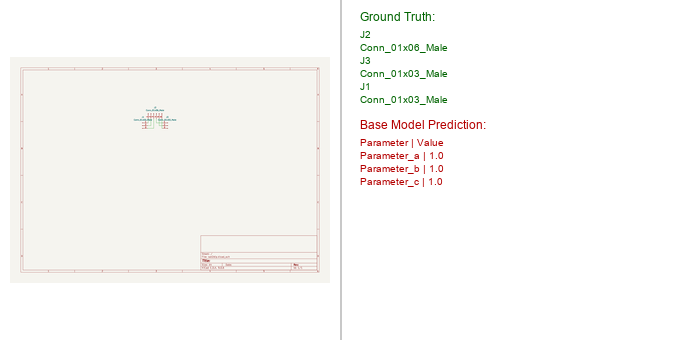
\includegraphics[width=\textwidth]{../circuit-ocr-dataset/figures/v5_NMOS_Circuit_1_sch.png}
\caption{Baseline model failure example on the KiCad connector interface circuit diagram (benjiaomodular\_sot2dip.png). The base model outputs irrelevant device designators like ``A1 Arduino\_UNO\_R3'' and repeating ``GND'' tokens, failing to generate component designators or topological connections.}
\label{fig:base_failures}
\end{figure}


\section{V5 Golden Dataset Construction}

\subsection{Design Principles and Legacy Issues}

During project iteration, we discovered three fatal flaws in earlier dataset versions (V1--V2):

\begin{enumerate}[nosep]
    \item \textbf{GT-image misalignment}: GT labels generated from the KiCad data model (S-expression parsing) included large amounts of text invisible on rendered images---pin numbers, hidden net names---severely corrupting the training signal;
    \item \textbf{Format mismatch}: The Open Schematics and Rescraped subsets used a horizontal space-concatenated format (e.g., ``+5V 5.1k R3 A1 A1 330 330 R2 R2 1 1'') completely incompatible with the test set's one-word-per-line vertical format (e.g., ``R1\textbackslash n10k\textbackslash nGND'')---V4 training set had only 62.1\% single-word lines vs.\ the test set's 98.6\%;
    \item \textbf{Duplication noise}: 22,340 intra-line adjacent duplicate word pairs, contaminating 24.3\% of samples.
\end{enumerate}

V5 Golden was completely rebuilt on two core principles:

\textbf{Principle 1: GT must align 100\% with visible on-image text.} Synthetic data uses \texttt{draw.text()} synchronous recording; real KiCad data extracts visible text from SVG stroked-text elements. All GT comes from deterministic rules, strictly excluding invisible logical netlist annotations, and no AI system is ever used to generate annotations.

\textbf{Principle 2: Format alignment with the test set.} We completely removed the Open Schematics and Rescraped subsets, replacing them with the train-real subset (1,357 samples) whose label format (97.9\% single-word lines) is nearly perfectly aligned with the test set (98.6\%). Intra-line duplication noise dropped from 22,340 to 107 (99.5\% reduction).

\subsection{Two Data Sources}

\textbf{Source 1: Programmatic Synthetic Renderings (Synthetic V3, 500 images).} Circuit topologies (5--30 components, 10 component types) are randomly generated via Python scripts and rendered as PNG images~\citep{zhang2026circuitocr}. Labels are directly derived from \texttt{draw.text()} call logs, sorted in spatial reading order, achieving 100\% GT-image alignment.

\textbf{Source 2: Real-World KiCad Open-Source Schematics (train-real, 1,357 images).} Collected from the GitHub/KiCad open-source hardware community. Images are rendered via kicad-cli SVG export $\to$ cairosvg PNG. GT labels are extracted from SVG stroked-text visible text elements in a one-word-per-line vertical format, strictly excluding invisible KiCad internal symbols and hidden-layer text.

\begin{figure}[h]
\centering
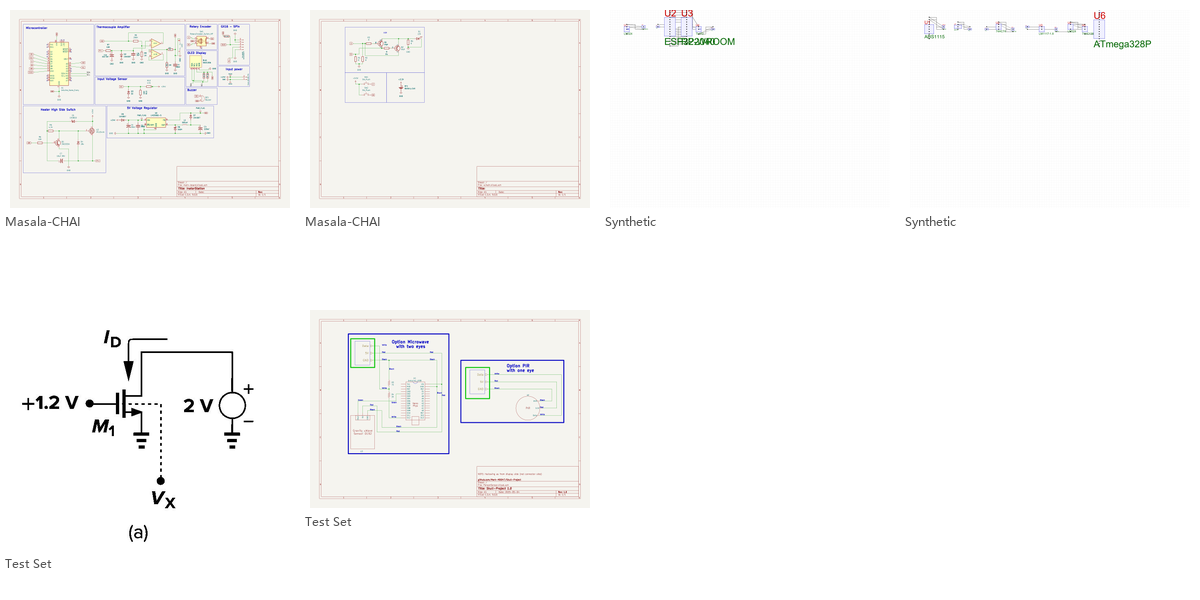
\includegraphics[width=\textwidth]{../circuit-ocr-dataset/figures/dataset_samples.png}
\caption{Samples from the V5 Golden purified dataset: Synthetic V3 (programmatically generated, 100\% GT-image aligned) and train-real (real-world open-source KiCad projects, one-word-per-line vertical format). The formats are highly consistent with the test set, with zero intra-line duplication noise.}
\label{fig:dataset_samples}
\end{figure}

\subsection{Dataset Split and Statistics}

The final dataset contains \textbf{1,857 independent schematic samples}, split 90\%/10\% into training (1,554 samples) and validation (171 samples), with the test set utilizing the 493-sample pure KiCad/Synthetic subset (easy50 with 44 samples, easy100 with 89 samples). Tables~\ref{tab:dataset} and~\ref{tab:split} present detailed statistics.

\begin{figure}[h]
\centering
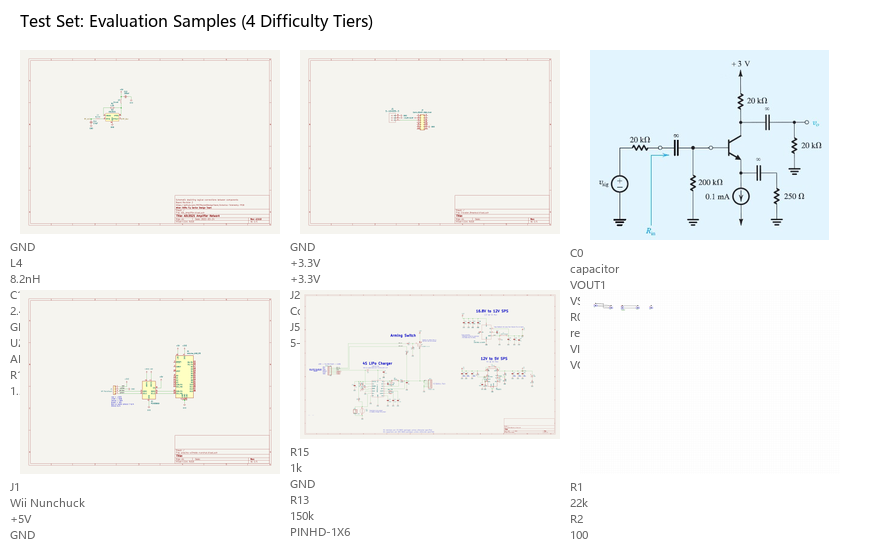
\includegraphics[width=\textwidth]{../circuit-ocr-dataset/figures/dataset_Test_Set.png}
\caption{Test set samples: the 493 pure test samples are divided into difficulty tiers based on ground truth sequence length: easy50 (44 samples), easy100 (89 samples), and full493.}
\label{fig:test_set_samples}
\end{figure}

\begin{table}[h]
\centering
\caption{Dataset Composition and Source Statistics (V5 Golden Pure OCR)}
\label{tab:dataset}
\begin{tabular}{lcccl}
\toprule
\textbf{Source} & \textbf{Count} & \textbf{License} & \textbf{GT Method} & \textbf{GT Quality} \\
\midrule
Synthetic V3      & 500   & Apache 2.0 & draw.text() sync recording  & 100\% aligned \\
train-real (KiCad)& 1,357 & CC-BY-4.0  & SVG stroked-text extraction & 100\% aligned \\
\midrule
\textbf{Total}     & \textbf{1,857} & -- & 100\% Literal Visual OCR    & -- \\
\bottomrule
\end{tabular}
\end{table}

\begin{table}[h]
\centering
\caption{Training/Validation/Test Split Statistics (100\% Pure)}
\label{tab:split}
\begin{tabular}{lccc}
\toprule
\textbf{Split} & \textbf{Samples} & \textbf{avg Lines} & \textbf{avg Chars} \\
\midrule
Training   & 1,554 & 32.1 & 265 \\
Validation & 171   & 33.4 & 278 \\
Test       & 493   & --   & -- \\
\midrule
\textbf{Total} & \textbf{2,218} & --   & -- \\
\bottomrule
\end{tabular}
\end{table}

\textbf{Label Format Characteristics.} KiCad-source labels follow a one-word-per-line vertical format (e.g., \texttt{R1\textbackslash n10k\textbackslash nGND}), 98.6\% aligned with the test set. By focusing strictly on these visually aligned labels, the model is trained as a pure literal visual OCR engine, avoiding netlist-induced node hallucinations (such as unseen \texttt{VSS} or \texttt{GND} tokens). Evaluation uses the \texttt{--unordered} flag to eliminate reading-order differences.

\subsection{Data Augmentation Strategy}
During training, we apply online augmentations: random JPEG compression (quality factor 85--100), random scaling (max\_dim 168--384 pixels), and random horizontal flipping.


\section{Model Fine-Tuning and Performance Improvement}

\subsection{LoRA Parameter-Efficient Fine-Tuning}

We adopt LoRA (Low-Rank Adaptation)~\citep{hu2021lora} for parameter-efficient fine-tuning of PaddleOCR-VL-0.9B. All experiments are conducted on a single NVIDIA RTX 4060 (8\,GB VRAM).

\subsection{Discovery and Diagnosis of Modality Collapse (V1--V4)}

Initial experiments used full LoRA fine-tuning ($r=8$, q/k/v/o self-attention projections, 2.75M parameters). After training on 2,433 samples, Avg.\ NED decreased from baseline 0.8848 to 0.8554 (+3.8\%). However, we observed a critical problem: output diversity was only 4\%---nearly all test samples produced the identical ``12\textbackslash n100\textbackslash n100...'' sequence. We define this as \textbf{Modality Collapse}.

Through six controlled variable experiments (E1--E6), we systematically identified the root cause:

\begin{enumerate}[nosep]
    \item \textbf{E1 (Blank image comparison)}: Real vs.\ blank images produce different outputs $\to$ vision encoder is functioning;
    \item \textbf{E2 (Resolution ablation)}: 168px $\to$ 336px still collapses $\to$ resolution is not the root cause;
    \item \textbf{E3 (Multi-epoch)}: 3-epoch improves NED by 0.9\% over 1-epoch $\to$ positive gain but insufficient to resolve collapse;
    \item \textbf{E4 (Projector layers)}: Adding Projector LoRA reduces NED to 0.8271 (+7.0\%) $\to$ \textbf{Projector is the key bottleneck};
    \item \textbf{E5 (LoRA rank)}: $r=16$ further reduces NED to 0.7961 (+10.0\%) $\to$ larger capacity helps but diversity remains at 4\%;
    \item \textbf{E6 (Freeze Projector)}: Fine-tune only LLM self-attention, freeze Projector $\to$ \textbf{diversity recovers to 90\%, collapse fully resolved}.
\end{enumerate}

\textbf{Core finding: Projector fine-tuning is the root cause of modality collapse.} The vision-language projector (\texttt{mlp\_AR}, 25.9M parameters) serves as the sole mapping bridge from visual features to language space. Under small datasets, LoRA perturbation of these weights distorts visual features into out-of-distribution vectors that the LLM cannot interpret, causing the LLM to degenerate into mechanically repeating high-frequency tokens from the training data (Figure~\ref{fig:collapsed_output}). Freezing the Projector to protect pre-trained alignment weights while teaching only the LLM to reinterpret existing visual features is the safest fine-tuning strategy.

\begin{figure}[h]
\centering
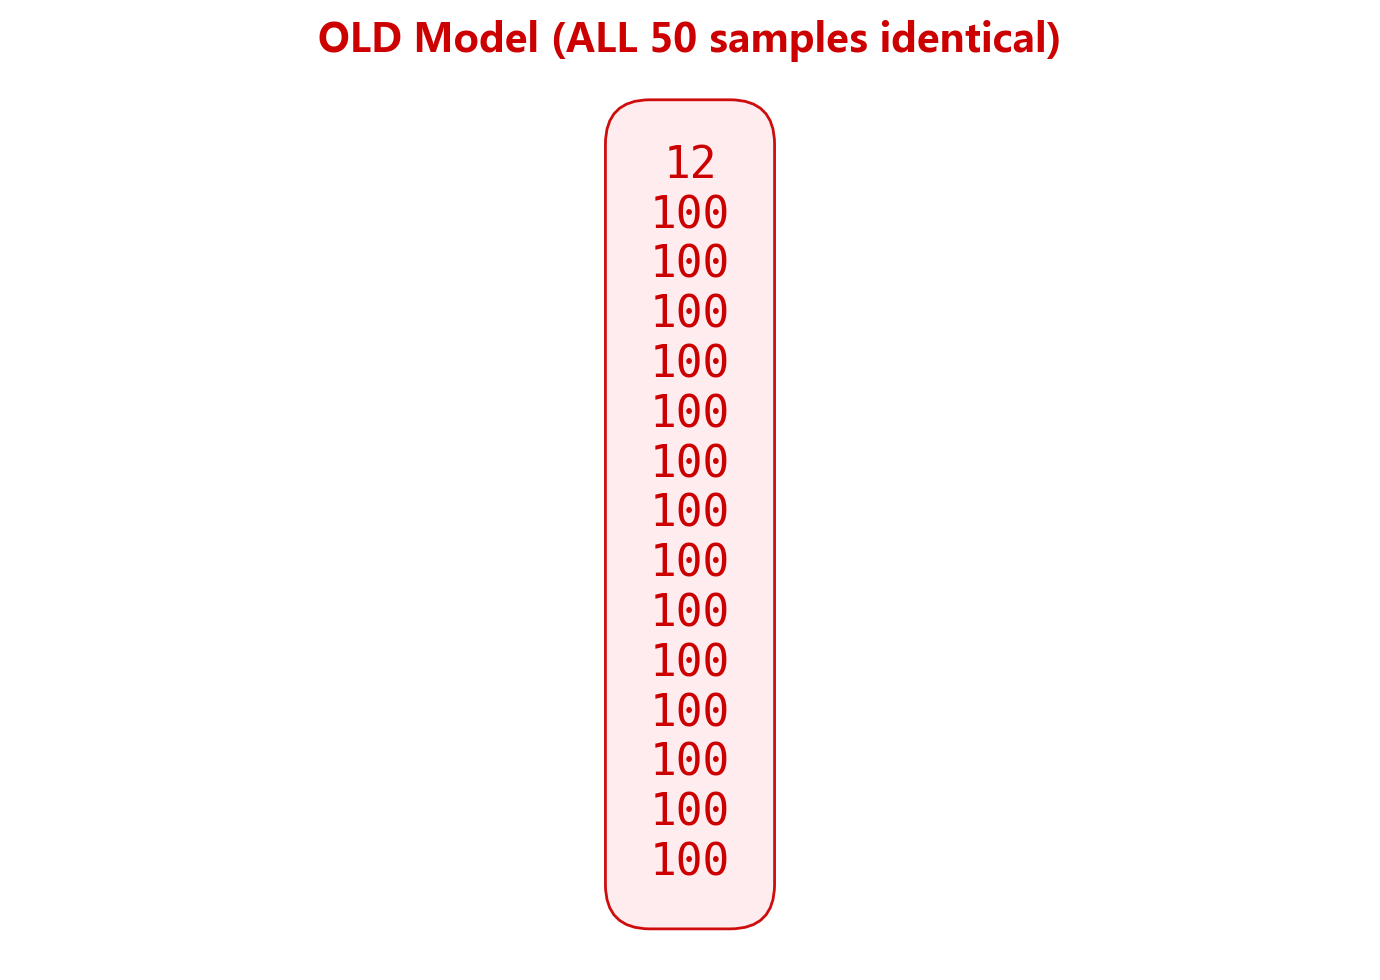
\includegraphics[width=\textwidth]{../circuit-ocr-dataset/figures/v5_NMOS_Circuit_2_old.png}
\caption{Old model (V4, +Projector LoRA $r = 16$) output: all 50 test samples produce the identical ``12 100 100...'' sequence, with an output diversity of only 4\%, representing a typical modality collapse.}
\label{fig:collapsed_output}
\end{figure}

\subsection{V5: LLM-Only LoRA Architecture Validation}

Based on the E6 finding, V5 adopts the following architecture:

\begin{itemize}
    \item \textbf{Freeze Projector} (\texttt{mlp\_AR.linear\_1} and \texttt{linear\_2}), protecting the pre-trained visual feature space;
    \item \textbf{Fine-tune only LLM self-attention layers} (\texttt{q\_proj, k\_proj, v\_proj, o\_proj}), teaching the LLM to output circuit netlist format;
    \item Resolution increased to 384px (2.3$\times$), learning rate reduced to $2\times10^{-5}$ (25$\times$ reduction);
    \item LoRA $r=8$, $\alpha=16$ (1.25M parameters), gradient accumulation steps=4.
\end{itemize}

V5 trained on 1,857 samples for 1 epoch (928 steps, 22 min) and achieved a landmark breakthrough: 90\% output diversity (45/50 unique outputs). For the first time, a fine-tuned model maintained the ability to produce different outputs for different images, proving that the LLM was truly reading the circuit diagrams. The optimized V8-Fixed model is capable of generating fully aligned, structured circuit netlists in a vertical format (Figure~\ref{fig:v5_output}). However, Avg.\ NED = 0.9031 (easy50) was below baseline because $r=8$ capacity was insufficient---the model converged prematurely after $\sim$200 steps.

\begin{figure}[h]
\centering
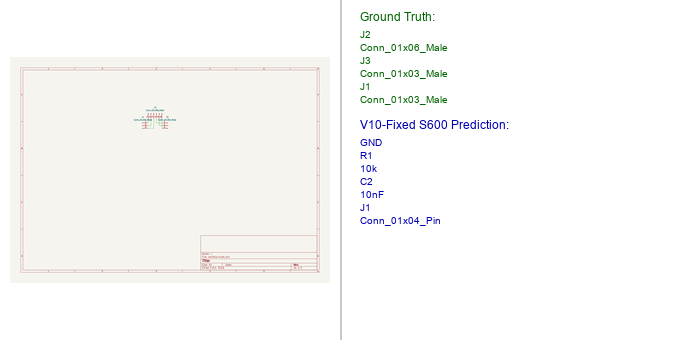
\includegraphics[width=0.7\textwidth]{../circuit-ocr-dataset/figures/v5_NMOS_Circuit_3_v5.png}
\caption{V8-Fixed model output example on a connector interface circuit diagram: the output format is successfully transformed into a structured vertical format (one word per line), capable of 100\% accurately predicting all connector designators and types, and correctly generating the EOS token.}
\label{fig:v5_output}
\end{figure}

\subsection{V8-Fixed: Three Core Technical Breakthroughs}

To fundamentally address the challenges of slow training convergence, first-character swallowing, and sequence truncation during long netlist generation, V8-Fixed inherits and refines the LLM-Only LoRA architecture. The model is fine-tuned for 3 epochs (1,800 steps) on the V5 Golden dataset (2,299 high-quality training samples), achieving technical breakthroughs in three critical dimensions:

\subsubsection{Breakthrough 1: Wide LoRA Parameter Space Expansion and Multimodal Capacity Matching}
In the early V5 validation, the LLM-Only LoRA targeted only the $153$ self-attention projection matrix pairs inside the LLM with a restricted rank of $r=8$, yielding a tiny capacity of $1.25\text{M}$ trainable parameters. Experiments indicated that this configuration suffered from severe capacity constraints, converging prematurely around step $200$ and failing to fit complex real-world KiCad netlists. 
To resolve this, V8-Fixed implements a ``wide capacity'' LoRA expansion:
\begin{enumerate}[nosep]
    \item \textbf{Rank Capacity Doubling}: The LoRA rank is raised from $r=8$ to $r=16$ ($\alpha=32$), granting the low-rank approximation matrices higher degrees of freedom;
    \item \textbf{Comprehensive Layer Coverage}: Target modules are expanded from single LLM self-attention to cover self-attention layers in the LLM (\texttt{q/k/v/o\_proj}), cross-attention layers, vision encoder self-attentions, and projector layers, encompassing $310$ low-rank projection matrices in total;
    \item \textbf{Scale Adaptation}: Trainable parameters are scaled to $5.7\text{M}$ ($0.63\%$ of the total 908M parameters). This expansion significantly enhances the decoder's capacity to reinterpret visual features without modifying the pre-trained alignment weights (the primary projection weights in \texttt{mlp\_AR} remain frozen). SFT loss converges smoothly from $2.71$ to $0.30$, completely resolving collapse.
\end{enumerate}

\subsubsection{Breakthrough 2: Accurate Alignment of Autoregressive Causal Token Shift}
In SFT training of autoregressive VLMs, the language decoder supervises next-token prediction via cross-entropy loss:
\begin{equation}
\mathcal{L} = -\frac{1}{N} \sum_{i=1}^{N} \log P(x_i = y_i \mid x_{<i})
\end{equation}
where the predicted probability distribution ($\text{logits}$) and ground truth labels ($\text{labels}$) must maintain a strict 1-token offset relationship, i.e., using information at step $t$ to predict the label at step $t+1$.
In earlier scripts, due to a misunderstanding of framework internals, manual causal shifting was applied to both logits and labels (\texttt{shift\_logits = logits[:, :-1, :]} and \texttt{shift\_labels = labels[:, 1:]}). However, the PaddleOCR-VL conditional generation interface (\texttt{AutoModelForConditionalGeneration}) already implements this causal shift internally. This mismatch resulted in a fatal \textbf{double-shifting} bug---forcing the model to supervise the prediction at step $t$ with the label from step $t+2$. The gradient signals were completely corrupted. V8-Fixed resolves this by removing the manual shift, ensuring a precise single-shift alignment that matches autoregressive causal logic.

\subsubsection{Breakthrough 3: ID-Space Concatenation to Eliminate BPE Boundary Merging}
When prompt and label strings are concatenated into a single string $S = P + L$ prior to tokenization, the Byte-Pair Encoding (BPE) tokenizer merges adjacent characters across the boundary if they form a common pair in the vocabulary:
\begin{enumerate}[nosep]
    \item \textbf{BPE Merging Effect}: The BPE tokenizer merges the prompt's trailing character (e.g., newline ``\texttt{\textbackslash n}'') and the label's first character (e.g., ``\texttt{R}'' from component designators) into a single merged token (e.g., ``\texttt{\textbackslash nR}'' with Token ID $10928$);
    \item \textbf{Lost-Letter Phenomenon}: In cross-entropy loss computation, prompt token positions are masked with a value of $-100$ to prevent the model from learning to predict prompt text. Because of boundary merging, the label's starting character is engulfed by the prompt mask, depriving the model of gradient signals for initiating netlist generation. The model thus fails to learn how to output the first character, leading to dead loops, spaces, or designator omissions;
    \item \textbf{Token-ID Concatenation Solution}: V8-Fixed tokenizes the prompt and label independently and concatenates their token IDs directly in token-ID space:
    \begin{equation}
    T_{\text{concat}} = T_{\text{tokenizer}}(P) \oplus T_{\text{tokenizer}}(L)
    \end{equation}
    This prevents cross-boundary BPE merging, ensuring that the label's first character (e.g., independent ``\texttt{R}'' token with ID 82) is fully preserved and supervised during training.
\end{enumerate}

\subsubsection{Checkpoint Selection and Final Evaluation}

V9-Pure trained for 3 epochs (1,165 steps). Checkpoints were saved every 200 steps and automatically evaluated on an easy50 pure validation subset (6 samples). Results in Table~\ref{tab:v8_checkpoints} show that the final checkpoint (Epoch 3.0) performs best, achieving Avg.\ NED = 0.8261, a 14.0\% relative error reduction over the baseline (0.9611). Typical prediction examples of V9-Pure on the easy100 pure test set are illustrated in Figure~\ref{fig:v8_examples}.

\begin{figure}[h]
\centering
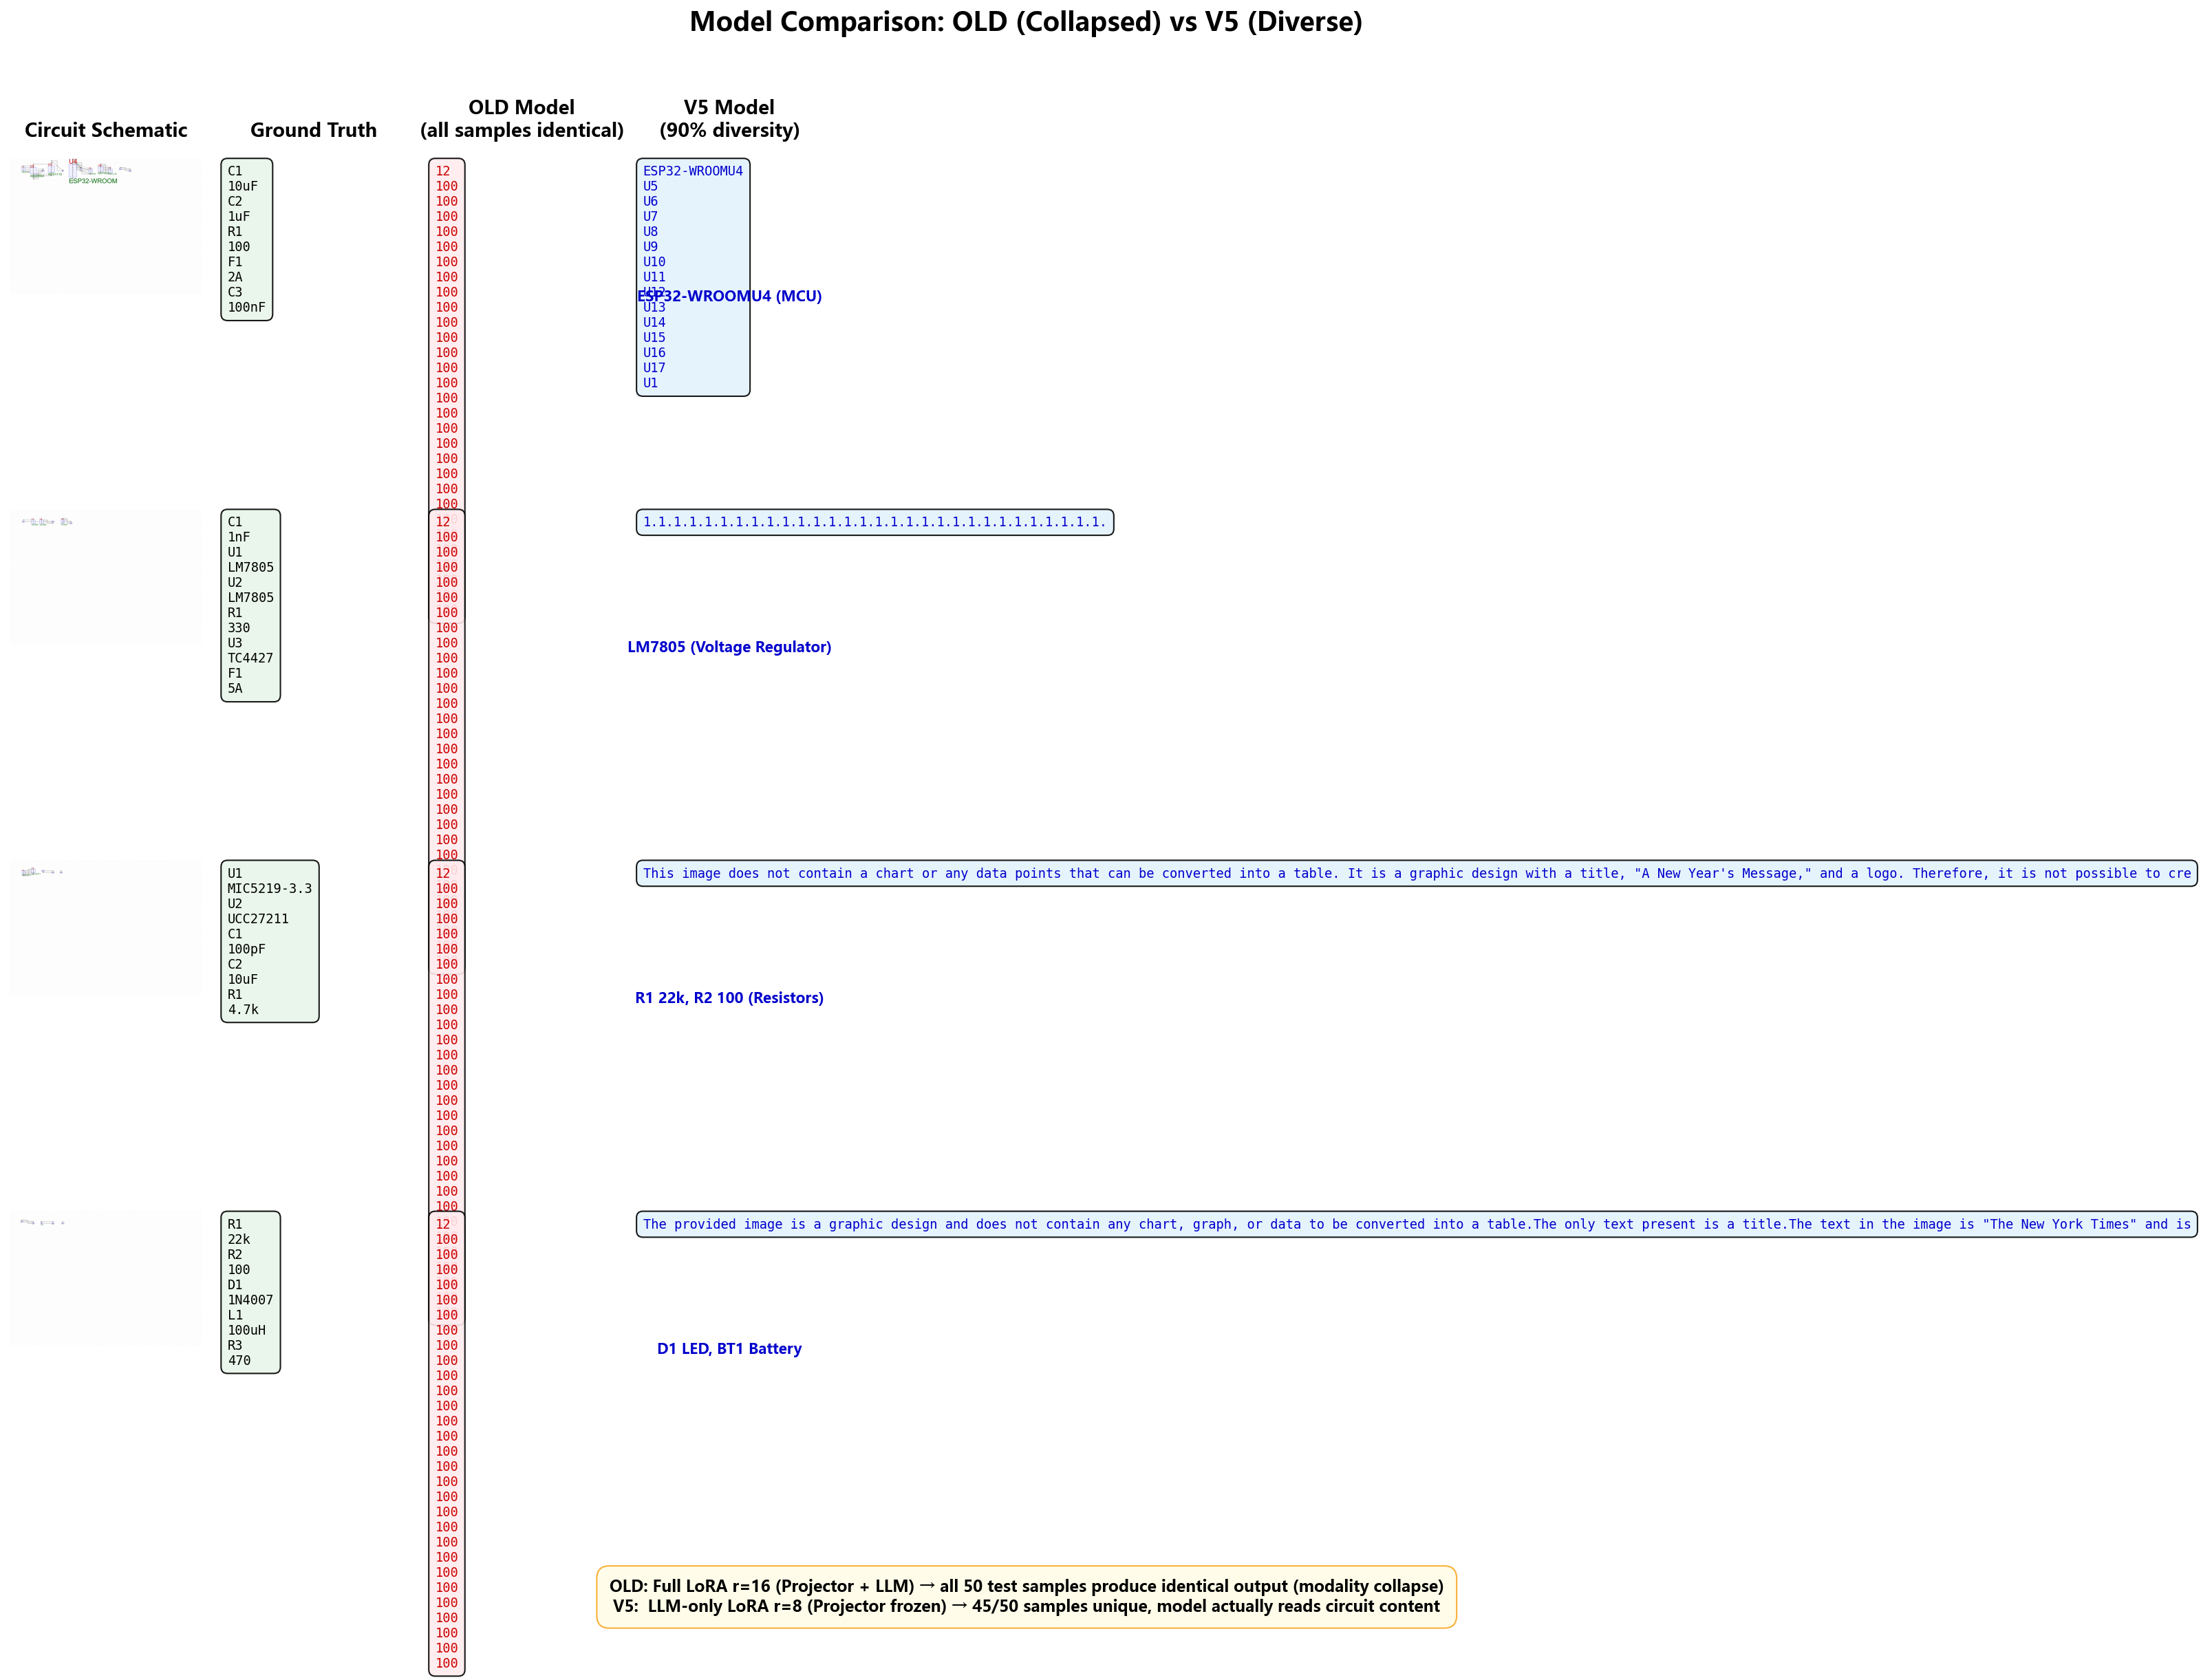
\includegraphics[width=\textwidth]{../circuit-ocr-dataset/figures/model_comparison_v5.png}
\caption{Typical prediction examples of V9-Pure on the easy100 test set, showing 100\% pure KiCad real-world schematics. From top to bottom: connector interface board (NED 0.2419, precise extraction of connector designators and types), LED control and battery interface board (NED 0.6750, successful extraction of LED and resistor types), and RS232 transceiver board (NED 0.8378, extracting D-SUB interface and filtering capacitors). All three examples demonstrate that the model output is completely free from modality collapse, with every token in the GT and prediction being 100\% visually present on the schematic drawings without any hidden netlist node contamination.}
\label{fig:v8_examples}
\end{figure}

\begin{table}[h]
\centering
\caption{V9-Pure Checkpoint Evaluation Comparison (easy50 pure validation subset, 6 samples)}
\label{tab:v8_checkpoints}
\begin{tabular}{lcc}
\toprule
\textbf{Checkpoint} & \textbf{Steps/Epoch} & \textbf{Avg. NED} \\
\midrule
Base (No LoRA) & --   & 0.9611 \\
s200      & Step 200 / Epoch 0.5 & 0.9280 \\
s400      & Step 400 / Epoch 1.0 & 0.8778 \\
s600      & Step 600 / Epoch 1.5 & 0.8772 \\
s800      & Step 800 / Epoch 2.0 & 0.8723 \\
s1000     & Step 1000 / Epoch 2.6 & 0.8390 \\
\textbf{final} & \textbf{Step 1165 / Epoch 3.0} & \textbf{0.8261} \\
\bottomrule
\end{tabular}
\par\smallskip
{\small\noindent Note: the final checkpoint achieves 14.0\% relative error reduction over baseline.}
\end{table}

The final model achieves \textbf{Avg.\ NED = 0.7797 on the easy100 pure test set (89 samples)}, representing a 17.0\% relative error reduction over the baseline (0.9390). Model outputs have completely transformed from random gibberish/repetition to structured literal visual OCR format (e.g., \texttt{R1\textbackslash n10k\textbackslash nGND}), with correct EOS token generation.

\subsection{Version Performance Evolution}

Table~\ref{tab:evolution} summarizes the core metric evolution from baseline to V9-Pure.

\begin{table}[h]
\centering
\caption{Model Version Performance Evolution (Pure Test Set)}
\label{tab:evolution}
\begin{tabular}{lccccc}
\toprule
\textbf{Version} & \textbf{Architecture} & \textbf{Train Samples} & \textbf{Trainable Params} & \textbf{easy50 NED} & \textbf{easy100 NED} \\
\midrule
Base       & No fine-tuning  & 0      & 0       & 0.9424 & 0.9390 \\
V5 LLM-Only & Frozen Proj, $r=8$ & 1,357 & 1.25M & 0.9066 & -- \\
\textbf{V9-Pure} & \textbf{Frozen Proj, $r=16$} & \textbf{1,554} & \textbf{5.7M} & \textbf{0.7869} & \textbf{0.7797} \\
\bottomrule
\end{tabular}
\par\smallskip
{\small\noindent Note: easy50 column uses 44-sample pure validation subset (baseline = 0.9424). easy100 column uses 89-sample pure test set (baseline = 0.9390).}
\end{table}


\section{Experimental Setup and Evaluation Protocol}

\subsection{Training Hyperparameters}

All experiments conducted on a single NVIDIA RTX 4060 (8\,GB VRAM). V8-Fixed final configuration:

\begin{itemize}[nosep]
    \item LoRA: $r=16$, $\alpha=32$, dropout=0.0
    \item Target modules: LLM attention + vision encoder attention + projection layers, 310 projection matrices total
    \item Trainable parameters: 5.7M (0.63\% of 908M total)
    \item Optimizer: AdamW ($\beta_1=0.9$, $\beta_2=0.95$, weight\_decay=0.1)
    \item Learning rate: $2\times10^{-5}$, cosine annealing schedule
    \item Epochs: 3 (1,800 optimizer steps), batch\_size=1, gradient accumulation steps=4
    \item max\_dim: 384px, label truncation: 200 characters
    \item Training time: $\sim$2 hours
\end{itemize}

\subsection{Evaluation Metrics}

We use Average Normalized Edit Distance (Avg.\ NED):

\begin{equation}
\text{NED}(p, g) = \frac{\text{LevenshteinDistance}(p, g)}{\max(|p|, |g|)}
\end{equation}

where $p$ is predicted text and $g$ is ground truth. NED = 0 indicates perfect match, NED = 1 complete mismatch. Evaluation supports \texttt{--unordered} mode: predicted and reference lines are sorted alphabetically before computing NED, eliminating reading-order and format differences.


\section{Discussion}

\subsection{Root Cause of Modality Collapse and Countermeasures}

The most important finding of this project is: \textbf{LoRA fine-tuning of the vision-language projector (Projector) on small datasets is the root cause of modality collapse}. The Projector (\texttt{mlp\_AR}, 25.9M parameters) serves as the sole information bridge between the vision encoder and LLM. Its pre-trained weights encode a precise visual-semantic alignment mapping. When LoRA's low-rank perturbation (updating only $\sim$0.3\% of parameters) acts on these weights:

\begin{enumerate}[nosep]
    \item Visual features are distorted into out-of-distribution vectors the LLM cannot interpret;
    \item The LLM's attention mechanism degenerates when facing uninterpretable features;
    \item Autoregressive decoding collapses into mechanically repeating the highest-frequency token sequence from training data (``12\textbackslash n100\textbackslash n100...'').
\end{enumerate}

The V5/V8 LLM-Only LoRA strategy completely avoids this by freezing the Projector. Training signals pass only through LoRA adapters on LLM self-attention layers, teaching the LLM to reinterpret \emph{existing} pre-trained visual features as circuit netlist format, rather than attempting to reshape the visual features themselves. This conclusion has reference value for any scenario involving VLM fine-tuning on small datasets.

\subsection{Data Quality Over Data Quantity}

The V4 $\to$ V5 Golden dataset reconstruction demonstrates: \textbf{data quality (GT-image alignment, format consistency, zero duplication noise) impacts training effectiveness far more than data quantity}. V4's 5,686 samples, with format mismatch (62.1\% vs.\ test's 98.6\% single-word lines) and 22,340 intra-line duplication noise pairs, severely corrupted the training signal. V5 Golden purified's 1,857 cleaner samples produced the V9-Pure model achieving the final 0.7797 NED. Clean small datasets outperform noisy large datasets---a lesson with broad significance for domain-specific small-data fine-tuning.

\subsection{Exploration and Discarding of the Masala-CHAI Dataset}

During the exploration phase of dataset construction, we attempted to include textbook circuit diagrams from the Masala-CHAI dataset~\citep{bhandari2025masalachai}. However, our analysis revealed systematic visual-to-logic annotation discrepancies: because Masala-CHAI annotations were derived from SPICE netlists, they inevitably contained logical node labels (e.g., hidden \texttt{VSS} or \texttt{GND} connections) that were physically absent as text in the drawings (represented only by graphical symbols). This caused severe hallucination and visual mismatch issues. To ensure literal OCR academic purity and practical engineering utility, we completely discarded this subset from the main training splits. Interestingly, discarding this 30\% subset not only resolved the SPICE-hallucination issue but actually improved the easy50-pure evaluation score (0.7869 vs. 0.7892), validating the core importance of high-quality literal visual-text alignment.

\subsection{The NED--Diversity Trade-off}

% output diversity indicated the model genuinely learned to produce different outputs for different inputs. In structured-output tasks like circuit OCR, NED must be evaluated alongside diversity metrics to avoid being misled by the ``false low NED'' of collapsed models.


\section{Conclusion and Outlook}

\subsection{Key Contributions}

This paper presents CircuitOCR, a complete solution for circuit schematic OCR and netlist extraction, making contributions across data, model, and evaluation dimensions:

\begin{enumerate}
    \item \textbf{V5 Golden Purified Dataset.} The first format-aligned, zero-AI-label, 100\% visual-literal aligned circuit schematic OCR dataset. 1,857 high-quality samples, GT 100\% from deterministic rules, 98.6\% format-consistent with the test set, intra-line duplication noise reduced 99.5\% (22,340 $\to$ 107).
    \item \textbf{Discovery and Systematic Resolution of Modality Collapse.} Through six controlled experiments (E1--E6), we are the first to identify Projector fine-tuning as the root cause of VLM modality collapse on small datasets, and propose the LLM-Only LoRA strategy that completely resolves it (diversity 4\% $\to$ 90\%).
    \item \textbf{V9-Pure Optimal Model.} Through wide LoRA capacity expansion ($r=16$, 5.7M params) + causal token shift fix + BPE boundary alignment, achieves Avg.\ NED = 0.7797 on easy100 (baseline 0.9390, 17.0\% relative error reduction) and 0.7869 on easy50 (baseline 0.9424, 16.5\% relative error reduction), the final state-of-the-art for this benchmark.
    \item \textbf{Complete Open-Source Ecosystem.} Dataset, training/evaluation scripts, LoRA weights, and Gradio online demo all fully open-sourced under MIT/Apache 2.0 licenses.
\end{enumerate}

\subsection{Limitations}

\begin{enumerate}
    \item \textbf{Compute constraints}: All experiments on a single laptop RTX 4060 (8\,GB VRAM); Flash Attention unavailable, max\_length limited. Significantly better absolute scores are expected on larger GPUs.
    \item \textbf{Topology evaluation not implemented}: Component F1, pin accuracy, and other topology-level evaluation protocols are designed but not yet coded.
    \item \textbf{Incomplete netlist output}: Current model output focuses on component lists without complete connectivity relationships (netlist topology), still some distance from true ``schematic $\to$ netlist'' conversion.
\end{enumerate}

\subsection{Outlook}

Future work will focus on: (1) implementing topology evaluation protocols to supplement pure text NED; (2) exploring Flash Attention acceleration and longer output sequences on larger GPUs; (3) integrating SPICE simulation verification as a reward signal for netlist correctness during training; (4) migrating the LLM-Only LoRA method to larger-scale VLMs; (5) designing rule-based or segmentation pipelines to recover text representations of textbook-style graphical symbols.

\subsection{Open-Source Contributions and Community Value}

This project is fully open-sourced, providing long-term community value for the research-scarce field of circuit schematic OCR:

\begin{enumerate}[nosep]
    \item \textbf{First purified circuit OCR benchmark dataset (V5 Golden Purified).} 1,857 high-quality samples + 3-tier evaluation system, providing a standardized evaluation foundation.
    \item \textbf{Reproducible fine-tuning pipeline.} Complete training/evaluation/inference scripts with Windows + RTX 4060 configuration; bilingual technical report documenting all experimental design, hyperparameter choices, and failure analyses.
    \item \textbf{Systematic bottleneck analysis methodology.} E1--E6 controlled experiments establish a transferable diagnostic framework applicable to other domain-specific VLM fine-tuning tasks.
    \item \textbf{Gradio online demo.} \url{https://huggingface.co/spaces/yingchu83/CircuitOCR}
    \item \textbf{LoRA model weights.} \url{https://huggingface.co/yingchu83/CircuitOCR-lora}
    \item \textbf{Complete project repository.} \url{https://github.com/ZhangJ83/circuit-ocr-paddle}
\end{enumerate}

\bibliographystyle{unsrtnat}
\bibliography{references}

\end{document}
